\documentclass[letterpaper]{article}

\date{Due: October 23, 11:59 pm}

\usepackage[margin=1in]{geometry}
% \usepackage{hyperref}
\usepackage[colorlinks]{hyperref}
\usepackage{capt-of}
\usepackage{amssymb}
\usepackage{amsmath}
\usepackage{url}
\usepackage{graphicx}
\usepackage{color}
\usepackage{bbm}
\usepackage{float}
\def\argmin{\mathop{\text{arg\,min}}}
\def\argmax{\mathop{\text{arg\,max}}}
\newcommand{\cov}{\mathrm{cov}}
\newcommand{\E}{\mathbb{E}}
% \newcommand{\argmax}{\mathop{\arg\max}}
% \newcommand{\argmin}{\mathop{\arg\min}}
\newcommand{\deriv}[1]{\frac{\partial}{\partial {#1}} }
\newcommand{\mbf}[1]{{\mathbf{#1}}}
\newcommand{\mbb}[1]{{\mathbb{#1}}}


%\newcommand{\sol}{1}


\begin{document}

{\centering
  \rule{6.3in}{2pt}
  \vspace{1em}
  {\Large
    CS589 Machine Learning - Fall 2019 \\
    Homework 4: Deep Learning \\
  }
  \vspace{1em}
  Due: October 23, 11:59 pm \\
  \vspace{0.1em}
  \rule{6.3in}{1.5pt}
}
\vspace{1pc}

%\maketitle

\paragraph*{Getting Started:} You should complete the assignment using your own installation of Python 3.6. Download the assignment archive from Moodle and unzip the file. This will create the directory structure as shown below. You will write your code under the Submission/Code directory. Make sure to put the deliverables (explained below) into the respective directories.

\begin{verbatim}
HW04
--- Data
    |-- Housing Prices Dataset
    |-- Reduced MNIST Dataset
    Code
    |-- Q1_Template.py
    |-- Q2_Template.py
--- Submission
    |--Code
    |--Figures    
    |--Predictions
\end{verbatim}

If you are stuck on a question consider attending the office hours.

\paragraph*{Data Sets:} 
\begin{enumerate}
    \item For question \ref{sec:linear} you will use housing retail prices dataset: Housing retail prices are influenced by numerous factors in addition to the number of bedrooms or lot area. The Housing Prices Dataset contains a multitude of explanatory variables and the final sales price of the houses. \vspace{12pt}
    
    \item For question \ref{sec:FC}, we'll use a subset of the MNIST dataset of handwritten digits containing 10 classes (digits 0-9). The first 100 digits (each 28x28 pixels) in the dataset are shown in the figure below.  \vspace{12pt}


\begin{table}[h!]
\center
\begin{tabular}{|l|c|c|c|c|c|}\hline
Dataset & Training Cases & Validation Cases & Test Cases & Dimensionality & Target \\\hline\hline
Housing Prices Dataset & 1500 & 500   & 900 & 240 & integer value \\\hline
Reduced MNIST Dataset & 10000 & 10000 & 10000 & 784 & 10 Classes (0-9) \\\hline
\end{tabular}
\end{table}
\begin{center}
    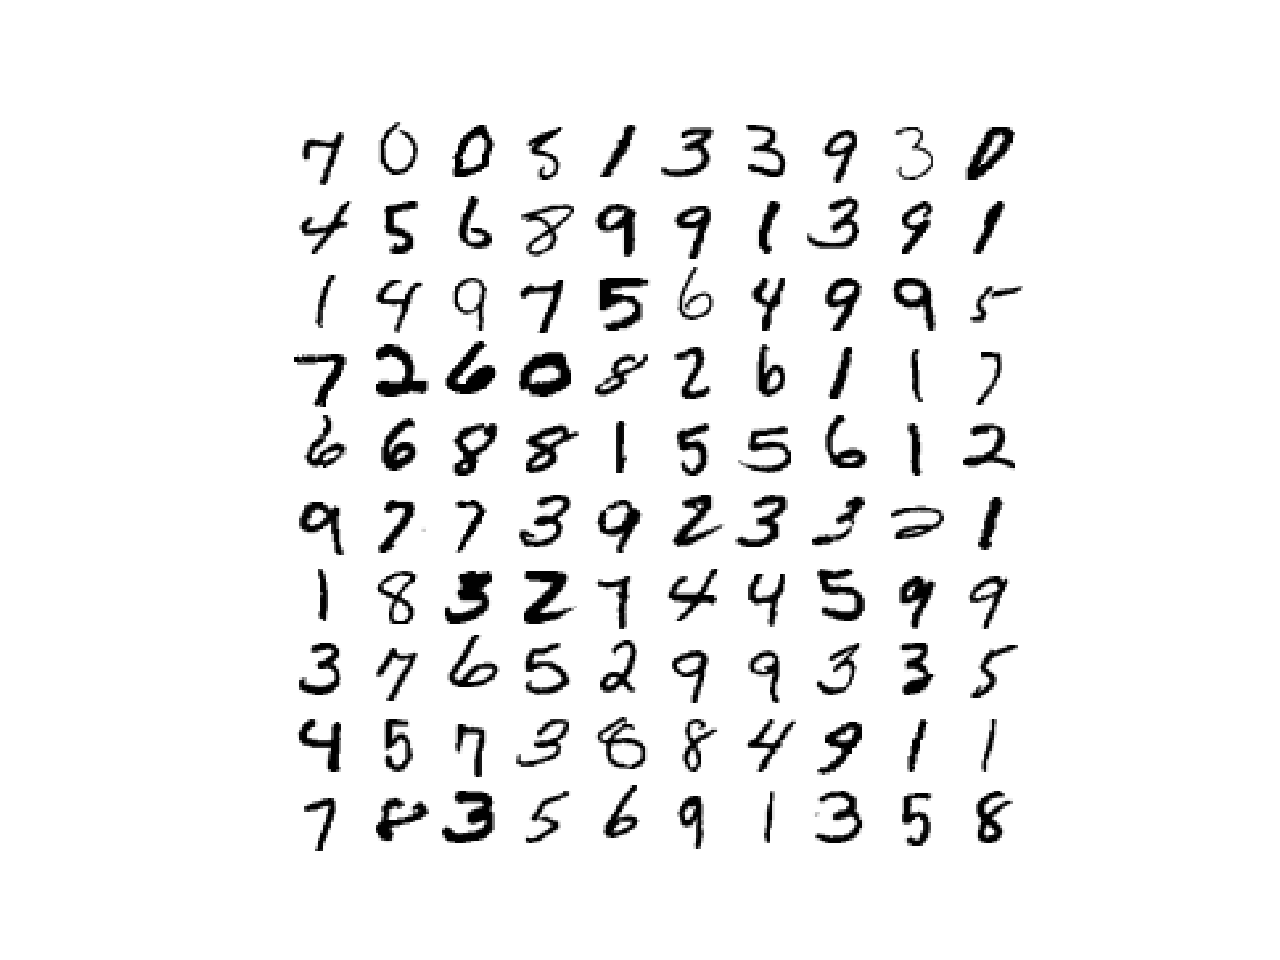
\includegraphics[scale=0.5]{mnist.png}
\end{center}
\end{enumerate}

\paragraph*{Deliverables:} This assignment has three types of deliverables: a report and code files. 
\begin{itemize}
\item \textbf{Report: } The solution report will give your answers to the homework questions (listed below). The maximum length of the report is 5 pages in 11 point font, including all figures and tables. You can use any software to create your report, but your report must be submitted in PDF format. 

\item \textbf{Code: } The second deliverable is the code that you wrote to answer the questions, which will involve training classifiers and making predictions on held-out test data. Your code must be Python 3.6 (no iPython notebooks, other formats or code from other versions). You may create any additional source files to perform data analysis. However, you should aim to write your code so that it is possible to re-produce all of your experimental results exactly by running \textit{python run\_me.py} file from the Submissions/Code directory. Remember to comment your code. Points will be deducted from your assignment grade if your code is difficult to reproduce!

\end{itemize}

\paragraph*{Submitting Solutions:} When you complete the assignment, place your final code in Submission/Code. If you used Python to generate plots then place them in Submission/Figures. Finally, create a zip file called `Submission.zip' from your `Submission' directory only (do not include `Data' directory). Only .zip files will be accepted for grading code (not .tar, .rar, .gz, etc.). You will upload your .zip file of code and your pdf report to Gradescope for grading. Further instructions for using Gradescope will be provided on Piazza and discussed in class.

\paragraph*{Academic Honesty Statement:} Copying solutions from external sources (books, web pages, etc.) or other students is considered cheating. Sharing your solutions with other students is  considered cheating. Posting your code to public repositories like GitHub is also considered cheating. Any detected cheating will result in a grade of 0 on the assignment for all students involved, and potentially a grade of F in the course.

\paragraph*{Note:} You may use \underline{scikit-learn} for question \ref{sec:linear} and \underline{PyTorch} for the model implementations in question \ref{sec:FC}  \\
\section{Linear Regression and Beyond [40 points + 10 Extra Credit]}
\label{sec:linear}

\begin{enumerate}
   
    \item {[10 points]} Ridge regression consists of finding the $w$ that minimizes $\left\|\mbf{y}-\mbf{X}\mathbf{w} \right\|_{2}^2 + \lambda \left\|\mbf{w}\right\| _{2}^2$, where the first term corresponds to the squared error in the regression estimation and the second is a regularization term. Here, $\mbf X\in\mathbb{R}^{N\times D}, \mbf w \in \mathbb{R}^D, \mbf y \in \mathbb{R}^N$. Show that the optimal $\mathbf{w}$ is $\mbf{w}^{*}=(\mbf{X}^T \mbf{X} + \lambda \mbf{I})^{-1} \mbf{X}^T \mbf{y}$, when the $\frac{\partial}{\partial \mbf{w}}$ of the loss function is zero.
    
    [Hint: You might want to use 2 important results of derivatives of matrix-vector products: \\$\deriv{\mbf z} (A\cdot z) = A^T$ and $\deriv{\mbf z} (\mbf z^T \cdot A \cdot \mbf z) = (A+A^T) \mbf z$.]
    
  
    \item {[5 points]} Linear regression models can be extended to capture non-linear relationships using basis function expansions. For the case in which a basis expansion $\mbf{x} \to \mbf{\Phi (x)}$ is used, how does the expression of $\mbf{w}^{*}$ change for Kernel Ridge Regression?\\
    
    \item {[Extra credit: 10 points]} Given a new sample $x_{new}$, show that the prediction $\hat{y} = (w*)^{T} \Phi(x_{new})$ can be written entirely in terms of inner products $\Phi (x_{i})^{T} \cdot \Phi (x_{\text{new}})$, and therefore computed using the kernel trick $k(x_{i}^{T}, x_{\text{new}})$.\\
    \textbf{Hint:} Using Matrix Inversion Lemma we can write: $$(\mathbf{X}^T \mathbf{X} + \lambda \mathbf{I})^{-1} \mathbf{X}^T \mathbf{y} = \mathbf{X}^T (\mathbf{X} \mathbf{X}^T + \lambda \mathbf{I})^{-1} \mathbf{y}$$
    

    \item {[25 points]} In some cases, considering linear dependencies suffices to capture the nature of the data, without the need of polynomial or RBF kernels etc. Using your choice of hyperparameter tuning method, run a simple \href{https://scikit-learn.org/stable/modules/generated/sklearn.linear_model.LinearRegression.html#sklearn-linear-model-linearregression}{\textbf{ordinary least squares (OLS) linear regression model}} on the Housing Prices Dataset. Then, train a \href{https://scikit-learn.org/stable/modules/generated/sklearn.linear_model.Lasso.html#sklearn-linear-model-lasso}{\textbf{lasso regression model}} and a \href{https://scikit-learn.org/stable/modules/generated/sklearn.linear_model.Ridge.html#sklearn-linear-model-ridge}{\textbf{ridge regression model}} on the dataset as well. Tune the hyper-parameters on the validation set and report the \href{https://scikit-learn.org/stable/modules/generated/sklearn.metrics.mean_absolute_error.html#sklearn-metrics-mean-absolute-error}{\textbf{mean absolute error}} on the test set for these three methods. 
    
    In addition, provide plots of the MAE vs. regularization constant for the lasso regression model and the ridge regression model (two plots total) as you vary the regularization constant using six or more reasonable values.
    
    You may use \underline{scikit-learn} for this question.
    \begin{table}[h!]
    \center
    \begin{tabular}{|l|c|c|c|}\hline
        & OLS         & Lasso       & Ridge    \\\hline
    MAE &             &             &          \\\hline
    \end{tabular}
    \end{table}
  
\end{enumerate}


\section{Fully Connected Neural Network [40 points]}
\label{sec:FC}

In this question, you will use \underline{pytorch} to implement a fully connected artificial neural network. You can find simple tutorials to get started with Pytorch library at \href{https://pytorch.org/tutorials/beginner/deep_learning_60min_blitz.html}{here} and \href{https://medium.com/biaslyai/pytorch-introduction-to-neural-network-feedforward-neural-network-model-e7231cff47cb}{here}. The architecture consists of an input layer, hidden layer $h_{1}$ with 64 nodes, hidden layer $h_{2}$ with 32 nodes, and an output layer for classification into C = 10 classes. The inputs are 28x28 images, resulting in 784-long input vectors (d = 784). Size and notation for weights and biases corresponding to the layers are provided below:

$$W_1, b_1: [h_1 \times d],[h_1]$$
$$W_2, b_2: [h_2 \times h_1], [h_2]$$
$$W_3, b_3: [C \times h_2],[C]$$

\textit{\textbf{Activations:}} 
\begin{enumerate}
    \item $ Sigmoid \ activation: \sigma(z) = \frac{1}{1 + e^{-z}}$
    \item $ReLU(z) = max(0,z)$
    \item $Softmax \ activation: softmax(z_i) = \frac{e^{z_i}}{\sum_{j=1}^{C}e^{z_j}}$
\end{enumerate}

\textit{\textbf{Note: For 2.1 and 2.2 and 2.3 we will be deriving the expressions assuming binary classification task because expressions are more simplified for binary classification task. In 2.3, for implementation, you need to implement the code for multi-class classification task on provided MNIST data with 10 labels. }}

\begin{enumerate}
\item{[6 points]} Given an input vector $\textbf{x} \in \mathbb{R}^{d}$, write an expression for the output of hidden layers $z^{(1)}$, $z^{(2)}$ and final output $\hat{y}$. For this question, assume a sigmoid activation is applied on the output of each hidden layer and on the final output layer. Write expression in terms of $x$, $W_1$, $b_1$ $W_2$, $b_2$, $W_3$, $b_3$, and sigmoid function $\sigma$. 

$$z^{(1)} = $$
$$z^{(2)} = $$
$$z^{(3)} = \hat{y} = $$

\item{[6 points]} For this question, assume that the classifier uses the binary cross-entropy loss for binary labels which is defined as:
 $$L(y,\hat{y}) = -(y \log(\hat{y})+(1-y)\ log(1-\hat{y}))$$
where $y$ denotes the correct label associated with the input $x$, and $\hat{y}$ denotes the output probability as derived in previous question.

% \textit{\textbf{Note:}} $\frac{d\sigma(z)}{dz} = \sigma(z)({1-\sigma(z)})$


First, derive the expression of the partial derivatives used for backpropagation. Write your expression in terms of $z^{(1)}$, $z^{(2)}$, $sigmoid  \ \sigma$ and $\hat{y}$\\
{\bf Hint:} The derivations for parts (a) and (b) are given as a hint please complete parts (c), (d) and (e).
\begin{enumerate}
    \item $$\frac{\partial{L}}{\partial{\hat{y}}} = $$\\
    {\bf Solution:} {\color{blue}  $$\frac{\partial{L}}{\partial{\hat{y}}} = -\frac{y}{\hat{y}} + \frac{(1-y)}{1-\hat{y}}$$}
    \item $$\frac{\partial{L}}{\partial{W_3}} = \frac{\partial{L}}{\partial{\hat{y}}}\frac{\partial{\hat{y}}}{\partial{W_3}} = $$
    {\bf Solution:} {\color{blue} $$\frac{\partial{L}}{\partial{W_3}} = (\hat{y} - y)(z^{(2)})^T$$}
    \item $$\frac{\partial{L}}{\partial{b_3}} = \frac{\partial{L}}{\partial{\hat{y}}}\frac{\partial{\hat{y}}}{\partial{b_3}} = $$
    \item $$\frac{\partial{L}}{\partial{W_2}} =  \frac{\partial{L}}{\partial{\hat{y}}}\frac{\partial{\hat{y}}}{\partial{z^{(2)}}}\frac{\partial{z^{(2)}}}{\partial{W_{2}}} = $$
    \item $$\frac{\partial{L}}{\partial{b_2}} = \frac{\partial{L}}{\partial{\hat{y}}}\frac{\partial{\hat{y}}}{\partial{z^{(2)}}}\frac{\partial{z^{(2)}}}{\partial{b_{2}}} = $$
\end{enumerate}

 
 \item{[6 points]} Now, derive the partial derivatives in 2.2 again, but with ReLU non-linearity for the hidden layers and sigmoid for the output layer.\\
 {\bf Hint:} The derivations for parts (a) and (e) are given as a hint please complete parts (b), (c) and (d).
 \begin{enumerate}
    \item 
    {\bf Solution for part a:} {\color{blue}  $$\frac{\partial{L}}{\partial{\hat{y}}} = -\frac{y}{\hat{y}} + \frac{(1-y)}{1-\hat{y}}$$}
    \item[(e)]
    {\bf Solution for part e:} {\color{blue} $$\frac{\partial{L}}{\partial{b_2}} = 
\begin{cases}
\left(W_3^T (\hat{y} - y) \right) & z^{(2)} > 0\\
0 & z^{(2)} \leq 0\\
\end{cases}
$$}
\end{enumerate}
 
 \item{[2 points]} How can you use the partial derivatives to optimize the neural network model? Explain the concept and write the update equation for parameters $W_3$ and $b_3$, assuming learning rate $\alpha$.

 \item{[20 points]} Now, implement the neural network with the architecture outlined above using PyTorch library for classifying MNIST digits, containing 10 output labels. In particular, you need to define your layers in the \texttt{\_\_init\_\_()} function, and define the connectivity between the layers in the \texttt{forward()} function of class \texttt{NNet(nn.Module)}. The hidden layers use ReLU activation and class probability output layer uses softmax activation.  For training, use batch size of 32, and Adam optimizer (\texttt{torch.optim.Adam}) with learning rate of 0.002 for 15 epochs. You may use the training code that is included in the template. Plot the training and test accuracy with respect to number of epochs of training.

\end{enumerate}



\end{document}


